
\chapter{Evaluation}


In this section we will take a retrospective look at the tool and its achievements. We observe some benchmarks ran against competitors as well as measure how well Gentoo has performed given the expected pre-requisites as set out earlier in this thesis. We will also attempt to given a qualitative evaluation of how well it has performed, given initial user feedback (beyond the quantitative analysis).

\section{Metrics of success}

To appropriately judge the success of the extension, we must have some quantifiable metrics, described below

\begin{enumerate}
	\item \textbf{Time to vulnerability} - As mentioned in \ref{limitations}, measuring the total time taken to perform a scan in this human driven context is unfair; the tool does not set a boundary on total scans unlike an automated scanner does. Measuring time taken is however a useful metric, so in order to not completely circumvent using time, another more appropriate metric is suggested - \emph{time to vulnerability}. This will be measured as the total number of seconds taken from the moment a scan is initiated (the user clicks the visual cue given by the tool), until the scan is finished. A scan may finish under two circumstances: a vulnerability has been successfully reported or detected (this may happen at the first attempt by the user, or at a later try when the tool has fuzzed some inputs during the Action Replay phase), or when the tool reports it could not find a vulnerability. These 2 conditions are bounded in terms of possible time taken, allowing the total time to be measured.
	
	\item \textbf{Interaction volume} - A metric that is sometimes found when evaluating automated scanners  is that of bytes sent and received by the application \cite{stateOfArtAutomatedBlackBoxWebAppVulnTesting}. This quantifies the impact the tool has when stressing the website by fuzzing inputs. The smaller this metric is, the more efficiently the tool is performing its job, by detecting vulnerabilities with fewer web requests sent.
	
	\item \textbf{Number of replays needed} - A similar metric to interaction volume, this number measures how many 'replays' are required by the tool to successfully detect a vulnerability. Both of these metrics measure the efficiency of the tool in detecting vulnerabilities, but this metric more accurately tests the efficiency of the fuzzing engine provided by the tool. Ideally, the tool uses the inputs which are known to work with higher success rates first, and the more esoteric fuzzes would come last, when there is already a decreased likelihood of them working anyway. It also encourages the tool to only include meaningful and relevant fuzzing techniques per vulnerability type, otherwise the tool \emph{could} theoretically fuzz forever. The fewer number of replays needed by the tool in order to find a vulnerability, the better it is performing.
	
	%	\item \textbf{Recommendation to vulnerability conversion rate} - An automated scanner is often measured in terms of how many false positives it shows, because it is expected to either positively or negatively declare the existence of a vulnerability. This would be an unfair means of benchmarking this extension - 
\end{enumerate}


\section{Experiments}


\subsection{Test benches}
In order to test our tool during development, it is not necessary to build a vulnerable web application from scratch. A much more bare bones approach was taken with the Test Harness, by building a page which presented the basic features of the vulnerabilities we were interested in exploiting. 
 %Not only would this be time consuming (beyond the purposes of building a tool to exploit such an application), it would also bias the ensuing development of the extension so that it is tailored to successfully detect every injected vulnerability in the web application.
  Fortunately, there already exist tools dedicated to this purpose. \\

As previously mentioned, DVWA is a vulnerable web application written in PHP, using MySQL for database interactions \cite{dvwaSite}. This application contains a good selection of predefined vulnerabilities to test against:
\begin{multicols}{3}
	\begin{itemize}
		\item Brute Force Login
		\item Command Execution
		\item CSRF
		\item File Inclusion
		\item SQL Injection
		\item Upload Vulnerability
		\item XSS	
	\end{itemize}
\end{multicols}

Another existing tool is WebGoat \cite{webgoatIntro, webgoatGithub}, supported by OWASP. This is an actively supported project by the open source community, and also contains a healthy amount of potential vulnerabilities for developers to test against:

\begin{multicols}{3}
	\begin{itemize}
		\item 	Access Control Flaws
		\item 	AJAX Security
		\item 	Authentication Flaws
		\item 	Buffer Overflows
		\item 	Code Quality
		\item 	Concurrency
		\item 	XSS
		\item 	Improper Error Handling
		\item 	Injection Flaws
		\item 	Denial of Service
		\item 	Insecure Communication
		\item 	Insecure Configuration
		\item 	Insecure Storage
		\item 	Malicious Execution
		\item 	Parameter Tampering
		\item 	Session Management Flaws
		\item 	Web Services
		\item 	Admin Functions
	\end{itemize}
\end{multicols}

Similarly to the above, there exist more testing tools of this kind, such as WackoPicko \cite{wackoPickoGithub} and HacmeBank \cite{hacmeBankMcAfee}. A more extensive list of existing applications of this kind has been produced by OWASP \cite{owaspVulnerableWebAppsList}. For the purposes of the experiments in this project, we will test against DVWA, WebGoat and WackoPicko, in order, as needed per vulnerability. This provides a good variety of implementations of vulnerabilities to test against; if the tool successfully finds the targeted vulnerabilities in these applications then it is likely to do well in other contexts.

\subsection{Test methodology}
The main method of testing my extension is to pit Gentoo against other existing automated vulnerability scanners. Some potential candidate scanners include \emph{OWASP ZAP} \cite{owaspZapPage}, \emph{w3af} \cite{w3af} and \emph{burpsuite} \cite{burpSuitePage}. All the scanners will analyse the aforementioned vulnerable applications used in testing. To avoid the case where the produced extension overfits its scanning model to the test vulnerable applications, this experiment will include more applications from the OWASP vulnerable web apps list \cite{owaspVulnerableWebAppsList}, not previously used in testing. \\

Since the browser extension makes use of user input, it is important to test the application with people of different security backgrounds. This relies on adequate classification in this group by the person undertaking the test. There will be 3 proposed categories of user experience when testing the tool; advanced, intermediate and beginner. An advanced user is expected to be well versed in web security, and have had prior experience in diagnosing (perhaps exploiting) vulnerabilities. An intermediate user may be someone getting to grips with this area, perhaps a student who is only now learning about these concepts, but hasn't \emph{necessarily} got experience in detecting or exploiting vulnerabilities. Beginner users are expected to be web savvy, people who are acquainted with using browsers and web applications, but are not necessarily interested or knowledgeable in web security. It is hoped that enough data is gathered to be able to have at least 5 unique people per suggested user group - it may be particularly hard to find advanced users that are willing to test the tool, whereas users who fit the other categories should be much easier to find. \\

To quantify how well the tool performs its job, the success rates of all 3 groups will be analysed when using the extension to find vulnerabilities. A very successful implementation of the project will have made it easy for non-experts to detect vulnerabilities, meaning that results from the beginner group would not vary very much from those in the intermediate and advanced groups using the tool. Therefore, inter-group vulnerability detection success rates will be analysed. From these success rates, it may be possible to extrapolate data on how educational the project was to users in the beginner and intermediate groups. This data could be further backed up by an additional quiz on whether the user has understood the type of vulnerability they detected, and whether they understand the ramifications of doing so by providing an example of a potential exploit they might design as a result. \\

Additionally, comparing each group success rate to the success rates of each of the automated scanners is useful to be able to validate the claim that a user driven, semi-automated approach is advantageous. This should be done within the context of what vulnerabilities the extension is able to detect - if an automated scanner can find more types of vulnerabilities than the ones the extension has been designed to find, then these will not be counted in the results. For a fair comparison in that aspect, it is assumed that with more development time, the extension may be developed further to be able to identify another type of vulnerability. \\

Another means of testing the success of the application would be to put it to test against real world applications. By activating the described passive mode as needed, and browsing web application domains, it is possible that a user of the extension finds vulnerabilities in the target application. Should this happen, it would be a great validating factor for the success of the tool.


\section{Benchmark analysis}

We now compare and analyse Gentoo's performance against other tools when scanning vulnerable web applications. We will be using OWASP's Zed Attack Proxy Project (\textit{ZAP}), and the Web Application Attack and Audit Framework (\textit{w3af}) as points of comparison - both of these are open source web scanners. In order to ensure a fair basis for comparing these tools, we used a virtual machine running the \textit{Kali} Linux distribution\footnote{ Kali version 3.26.2. The virtual machine was allocated 3.9GB memory, using an Intel i7-4980HQ at 2.8GHz (2 cores)} and installed each tool in this VM. \\

 As part of setting up these benchmarks (which were mostly geared towards finding XSS vulnerabilities as per Gentoo's current functionality), it was also necessary to use a proxy to disable the browser's XSS Auditor. Since the benchmarks are comprised of web applications with intentionally vulnerable functionalities, we want to observe this functionality without the extra protections added by the browser. For this purpose, we use BurpSuite's proxying feature to capture requests and disable the \texttt{X-XSS-Protection} header (should it be present, Figure \ref{fig:burp_xss_disabled}). We enable its use in Chrome by linking it with \textit{ProxySwitchOmega} \footnote{ ProxySwitchOmega is a Google Chrome extension to enable request proxying: https://goo.gl/iFSJvH.}. \\

\begin{figure}[h]
	\centering
	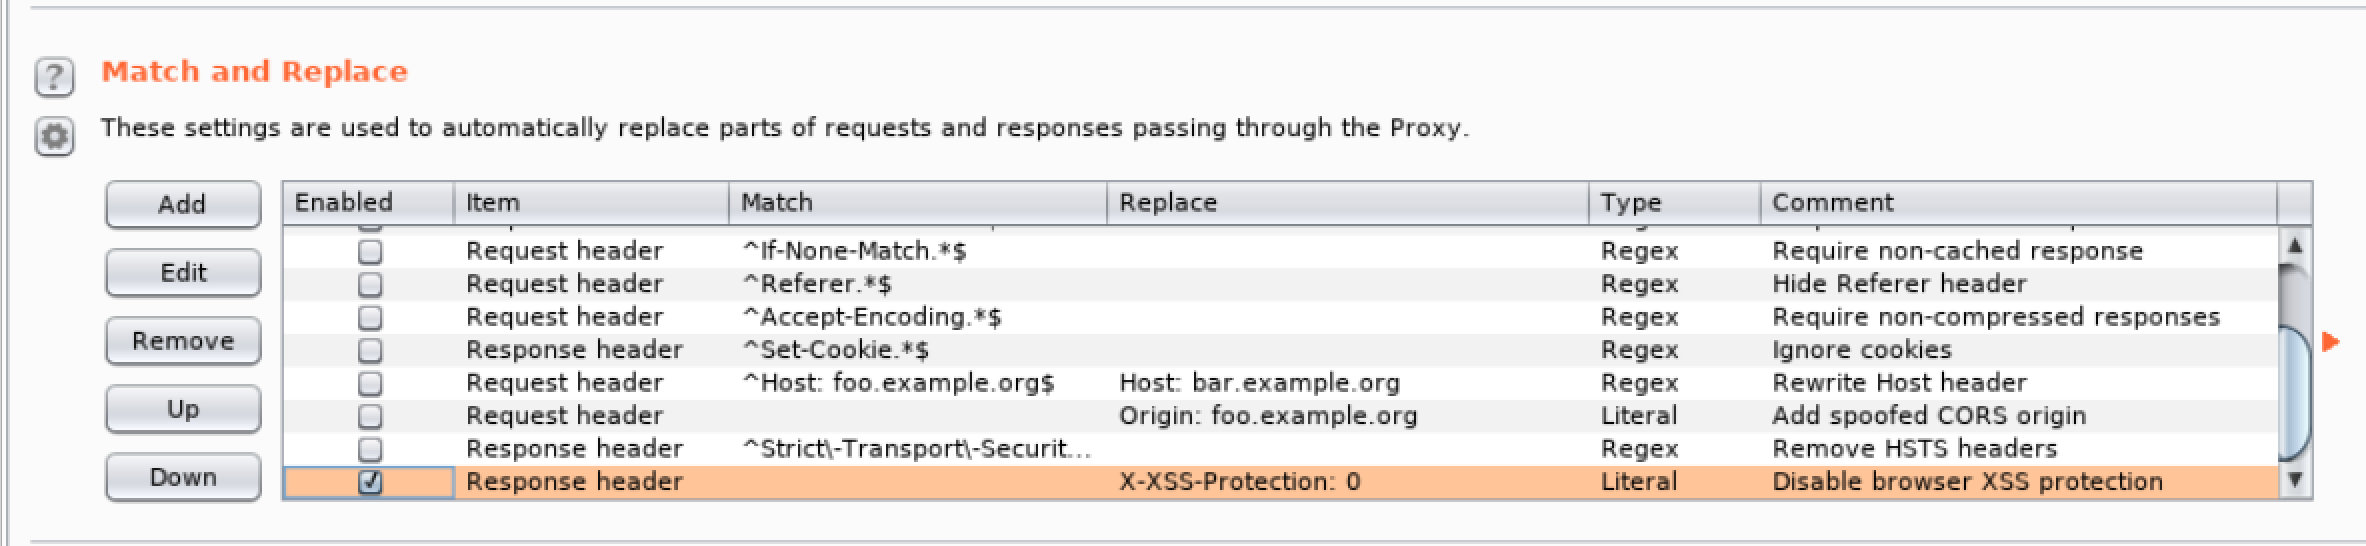
\includegraphics[width=\textwidth]{images/evaluation/burp_xss_disabled.png}
	\caption{Any request passed to Gentoo or the other tools is stripped of the \texttt{X-XSS-Protection} header, allowing for accurate XSS detection.}
	\label{fig:burp_xss_disabled}
\end{figure}

As explained before, we will be extracting 3 key metrics: \textit{Time to Vulnerability}, \textit{Interaction Volume} and \textit{Number of Attacks needed}. \textit{Time to vulnerability} is measured as the time from the moment the scan is initiated until the first 'vulnerability' is detected by the application (irrespective of whether this is the vulnerability we are specifically looking for or not - we will explain the reasoning for this later). \textit{Interaction Volume} is measured as the total number of bytes used in the scan by the tool. \textit{Number of attacks needed} measures how many requests a tool had to make before finding its first vulnerability in the scan (as a proportion to how many requests it made in the scan overall). \\ 

In order to extract data for the purposes of these experiments, we use console logging in Gentoo to acquire accurate timestamps for key events in a scan. For the other tools, we use the provided reporting and exporting functionalities by each tool and analyse the outputs of these to acquire the necessary data. \\

\subsection{Test Harness}

Firstly, we benchmarked the tools against the produced Test Harness. We ran Gentoo using the Action Replay functionality to detect the XSS vulnerabilities present in this page, and subsequently used the Passive Mode to scan the headers in the Test Harness. For ZAP, we used the \textit{Launch Browser} feature to crawl the page, and subsequently attacked it with all selected input vectors. We used the \textit{full\_audit} profile provided by w3af to perform the corresponding scan. \\

\begin{table}[h]
	
{\rowcolors{3}{green!24}{white}

	   \captionsetup{justification=centering}
	
	\caption{Running the tools against the Test Harness. The * by the \textit{Time to Vulnerability} column indicates the desired vulnerability (XSS) was not detected}
		\label{table:test_harness_benchmarks}
\begin{tabular}{ |p{4cm}||p{1.4cm}|p{1.4cm}|p{1.6cm}|p{2cm}|p{2cm}| }
	\hline
	\multicolumn{6}{|c|}{\textbf{Test Harness Benchmarks}} \\ [0.5ex]
	\hline \hline 
	Tool Being Tested& Time To Vulnerability & Total Scan Time & Interaction Volume & Attacks to Vuln / Total Attacks & \% of scan to 1st vuln \\
	\hline
	Gentoo (XSS detection)    & 9.6s      & 15.8s    & 32KB & 10/27 &37\% \\
	Gentoo (Header Analysis) & 50ms    &  3.0s    & 4KB&  1/4 &25\%\\
	ZAP                                   & 5.6s (*) & 7.8s      &  1.31MB &1621/2140 &76\%\\ 
	w3af                                 & 7.9s  (*) & 136.2s & 950KB & 71/1126 &6.3\%\\
	\hline
\end{tabular}
} \\
\end{table}

Table \ref{table:test_harness_benchmarks} shows how each tool performed when measured up against the aforementioned metrics. For the XSS detection in Gentoo, we intentionally measure the time taken by a human to interact with the extension to analyse the outputs produced. The scan begins once the Action Replay recording begins, which means a form input must be manually submitted, the Action Replay button clicked on the new page, and each of the resulting attacks inspected for vulnerabilities. The scan is considered to be finished once the last successful attack has been registered as an observable output in the extension (at the same time the extension badge icon turns to an exclamation mark (\textbf{!})), or, in the absence of a vulnerability, once the user has finished inspecting the attacks. \\

In this case, 2 separate attacks were successful in triggering an XSS vulnerability during the extension's scan. It took the user a relatively short time to come to this conclusion, as the scan only took around 16 seconds. This seems especially successful when compared to the other automated results - ZAP's scan was about half the time, whilst w3af's was unusually long, and neither of these seemed to have correctly found the XSS flaw on the page. The order in which attacks were performed seemed to be good, with the first vulnerability being reported when the Gentoo scan was only about 37\% of the way through. In comparison to the other tools, it is clear both by the number of requests and the interaction volume that Gentoo did this with a significantly lower number of requests. This could be due to overfitting and creator's bias however, as the Test Harness was heavily used alongside the development of Gentoo. We will bear this in mind as we look at other vulnerable pages shortly.  \\

When producing this data, it became evident that comparing Gentoo to these tools on a basis of whether they had found a specific vulnerability on an application seemed unfair. As it stands, our extension is very focused on finding a given vulnerability, and if set up correctly, seems to provide good feedback on said vulnerability. However, ZAP and w3af are stand-alone implementations designed to run without user interaction, and as such, will scan the entire web-application in a non-discriminatory way when it comes to selecting vulnerabilities - anything of use is flagged up for the final report. Thus, although we set up these tests in a manner such that Gentoo \textit{should} find a vulnerability it has been designed to catch, we will not hold it against the results of the other 2 should they find other useful information along the way. \\

In the benchmark above (Table \ref{table:test_harness_benchmarks}), neither ZAP nor w3af reported an XSS vulnerability for the Test Harness. This is perhaps a little odd, as the page containing this vulnerability conforms to the minimum requirements for a Reflected XSS. However, since it is a \textit{very} simple page, it could be supposed that the page is not complex enough for the filters being used by the other scanners to correctly classify it as vulnerable to XSS. \\

Nonetheless, all 3 of the tools produced warnings when analysing the application headers. With the exception of w3af, the tools seem to clearly indicate whether the results are being passively obtained or not. However, when observing the scan, the speed at which the alerts in w3af are produced seems to indicate that internally, these are still acquired passively from web requests. \\

\begin{table}[h]
	
	{\rowcolors{3}{green!24}{white}

		\captionsetup{justification=centering}
		
		\caption{The alerts produced by the different tools when analysing the Test Harness}
		\label{table:test_harness_alerts}
		\begin{tabular}{ |p{7cm}|>{\centering\arraybackslash}m{2cm} |>{\centering\arraybackslash}m{2cm} |>{\centering\arraybackslash}m{2cm}| }
			\hline
			\multicolumn{4}{|c|}{\textbf{Test Harness passive alerts}} \\ [0.5ex]
			\hline \hline 
			Alert Type & Gentoo & ZAP & w3af \\
			\hline
			X-Frame-Options (Clickjacking) & X & X & X \\
			X-XSS-Protection & X & X & \\
			X-Content-Type-Options& X & X & \\
			Content-Security-Policy & X & & \\
			Referrer-Policy & X & & \\
			Strict-Transport-Security & X  & & \\
			Server Header Exposed & & & X\\
			DNS Wildcard config & & & X \\
			Too many HTTP methods allowed & & & X\\
			
			\hline
		\end{tabular}
	} \\
\end{table}

In Table \ref{table:test_harness_alerts}, we see that all of tools can agree that clickjacking is a big enough concern that the \texttt{X-Frame-Options} header should be set. We will ignore the alerts for the missing \texttt{X-XSS-Options} header because this is by design as previously explained, although it is interesting to note that w3af did not report this missing header in its scans. Some of the uniquely reported headers by Gentoo are also more recent additions - both the \texttt{Content-Security-Policy} and the \texttt{Referrer-Policy} are newer headers. As for the last 4 on the Table, these settings are more suggestions than alerts - these are flagged up by Gentoo and w3af, but do not necessarily indicate weaknesses. They are nonetheless useful in the \textit{information gathering} phase of any pentester, and shouldn't be readily ignored. \\ 

\subsection{DVWA}

We now proceed to look at how these tools perform at a more homogenous level by benchmarking them against a third-party produced application. \\
\begin{table}[h]
	
	{\rowcolors{3}{green!24}{white}

		\captionsetup{justification=centering}		
		\caption{Running the tools against DVWA.}
		\label{table:dvwa_benchmarks}
		\begin{tabular}{ |p{4cm}||p{1.4cm}|p{1.4cm}|p{1.6cm}|p{2cm}|p{2cm}| }
			\hline
			\multicolumn{6}{|c|}{\textbf{DVWA Benchmarks}} \\ [0.5ex]
			\hline \hline 
			Tool Being Tested& Time To Vulnerability & Total Scan Time & Interaction Volume & Attacks to Vuln / Total Attacks & \% of scan to 1st vuln \\
			\hline
			Gentoo (Reflected XSS)    & 6.6s      & 9.4s    &   66.3KB          & 4/15 & 27 \% \\
			Gentoo (Persisted XSS)    &  -- & 5.3s & 80.6KB & 13/13 & 100 \% \\
			Gentoo (Header Analysis) & 27ms    &  3.0s    & 17.9KB   &  2/5 & 40\%\\
			ZAP                                  & 2.6s & 66.6s     &  65.79MB & 3852/22995& 16.7\%\\ 
			w3af                                 & -- & -- & -- & -- &-- \\
			\hline
		\end{tabular}
	} \\
\end{table}

Once again, the results for the Gentoo XSS detection seem promising - the scan duration in DVWA is still very reasonable, even accounting for human interaction delays. The attack order is also effective, as the first confirmed vulnerability is found after just a quarter of the attacks are performed. However, Gentoo's search for a persisted XSS failed in the page containing that vulnerability. None of the attacks forged against this page worked - for a very simple reason. The Persistent XSS vulnerability in DVWA involves submitting a \texttt{textarea} - a form input that isn't designated by the \texttt{input} HTML tag. This is an oversight in Gentoo's page injection logic, as \texttt{textarea}'s are perfectly valid inputs to submit. However, this concern had not been addressed before this benchmark, negatively affecting Gentoo's evaluation. Unfortunately, we weren't able to configure w3af to successfully scan DVWA. w3af does possess authentication enabled scans and crawls as a feature, but we were unable to configure it in such a way that it could log into DVWA as a user as part of its crawl. The resulting crawl was very debilitated as a result - only very few resources that were not hidden behind the login form were accessible, and so we could not count this towards w3af's overall performance. In this benchmark, ZAP has performed very well. It executed close to 23 thousand requests in just over a minute, and detected its first serious vulnerability in only 2.6 seconds. This is an example where automated scanners can boast of their alacrity - all the while performing over 1500x more requests than Gentoo, it still found a vulnerability faster than a human could. \\

Table \ref{table:dvwa_alerts} highlights this further. During this time, ZAP has not only detected a Reflected XSS, but also Persisted XSS and other severe vulnerabilities - Path Traversals and SQL injections. At this point it's worth mentioning that Gentoo's passive mode, as with the Test Harness, has detected and warned the user about the same set of headers as ZAP has, with some more warnings added over ZAP. Both also found that the valuable \texttt{PHPSESSID} cookie should have probably been set with the \texttt{httpOnly} flag to maximise session security. In this respect, both scanners have done well - ZAP has used the extra time of its scan to find important and relevant vulnerabilities. Its scan time is still over 5 times the duration of the combined Gentoo scans, so this success should almost be expected in an application such as DVWA, which is brimming with vulnerabilities.



\begin{table}[h]
	
	{\rowcolors{3}{green!24}{white}
		
		\captionsetup{justification=centering}
		
		\caption{The alerts \& warnings produced by the different tools when analysing DVWA. Those with ** are real, dangerous vulnerabilities found in DVWA}
		\label{table:dvwa_alerts}
		\begin{tabular}{ |p{7cm}|>{\centering\arraybackslash}m{2cm} |>{\centering\arraybackslash}m{2cm} |>{\centering\arraybackslash}m{2cm}| }
			\hline
			\multicolumn{4}{|c|}{\textbf{DVWA alerts}} \\ [0.5ex]
			\hline \hline 
			Alert Type & Gentoo & ZAP & w3af \\
			\hline
			XSS (Reflected) ** & X & X & --\\
			XSS (Persistent) ** &  & X & --\\
			Path Traversal ** &  & X & --\\
			SQL Injection **& & X & --\\
			X-Frame-Options (Clickjacking) & X & X & -- \\
			X-XSS-Protection & X & X & --\\
			X-Content-Type-Options& X & X &-- \\
			Content-Security-Policy & X & &-- \\
			Referrer-Policy & X & & --\\
			Strict-Transport-Security & X  & & --\\
			PHPSESSID Cookie Insecure Flags & X & X & -- \\
			\hline
		\end{tabular}
	} \\
\end{table}



\subsection{WebGoat}

Moving on, we now observe how each of the tools performs when scanning WebGoat, OWASP's deliberately insecure application designed to teach security lessons. Unfortunately, we still couldn't configure w3af to sign into WebGoat. As a result, it could still not perform any relevant scanning besides passive header analysis for alerts and warnings, and as such, it is not included in the following results. Surprisingly, Gentoo is unable to perform the Action Replay on this application. Although it can visually start a scan, under these circumstances, the \texttt{DevTools} script cannot identify the WebGoat page to be the active tab, resulting in an exception which does not allow the Action Replay algorithm to complete. As a result, only Gentoo's Passive mode worked as normal, acquiring weak header and cookie data as before. ZAP managed to complete another full application scan; using it's \textit{Launch Browser} feature, we were able to log into a user profile during testing, and emulate and crawl the application while it is still open. Once we are happy with the crawling done, ZAP then performs several attacks based off of this information. \\

\begin{table}[h]
	
	{\rowcolors{3}{green!24}{White}
		\captionsetup{justification=centering}		
		\caption{Running the tools against WebGoat}
		\label{table:webgoat_benchmarks}
		\begin{tabular}{ |p{4cm}||p{1.4cm}|p{1.4cm}|p{1.6cm}|p{2cm}|p{2cm}| }
			\hline
			\multicolumn{6}{|c|}{\textbf{WebGoat Benchmarks}} \\ [0.5ex]
			\hline \hline 
			Tool Being Tested& Time To Vulnerability & Total Scan Time & Interaction Volume & Attacks to Vuln / Total Attacks & \% of scan to 1st vuln \\
			\hline
			Gentoo (XSS detection)    & --     & --    &   --          & -- & -- \\
			Gentoo (Header Analysis) &  3.2s   & 6.2s   & 1.3MB   & 1/3 & 33.3\%\\
			ZAP                                   & 12.9s &  48.5s   & 68.0MB  & 1213/4437 & 27.3\%\\ 
			w3af                                 & -- & -- & -- & -- & -- \\
			\hline
		\end{tabular}
	} \\
\end{table}


Gentoo's header analysis is again very terse, as it picks up relatively few requests in order to analyse the necessary headers - the first vulnerability is found in the first of these. The interaction volume this time however is significantly larger, as WebGoat generates a lot more data per request than the other applications thus far. In the meantime, ZAP remains a consistent opponent by delivering a hefty scan in a reasonable time - under a minute. This is enough time to reel in 4 serious vulnerabilities, which the other tools have missed out on by lack of compatibility. Gentoo's header analysis still picks up on valuable session ID cookies and alerts to their lack of security, as does ZAP. 

\begin{table}[h]
	
	{\rowcolors{3}{green!24}{white}
		
		\captionsetup{justification=centering}
		
		\caption{The alerts \& warnings produced by the different tools when analysing WebGoat. Those with ** are dangerous vulnerabilities found in WebGoat}
		\label{table:webgoat_alerts}
		\begin{tabular}{ |p{7cm}|>{\centering\arraybackslash}m{2cm} |>{\centering\arraybackslash}m{2cm} |>{\centering\arraybackslash}m{2cm}| }
			\hline
			\multicolumn{4}{|c|}{\textbf{WebGoat alerts}} \\ [0.5ex]
			\hline \hline 
			Alert Type & Gentoo & ZAP & w3af \\
			\hline
			XSS (Reflected) ** & -- & X & --\\	
			SQL Injection **& -- & X & --\\
			XSS (Reflected in JSON Response) ** & -- & X & -- \\
			Parameter Tampering **& -- & X & --\\
			X-XSS-Protection & X & X & --\\
			Content-Security-Policy & X & &-- \\
			Referrer-Policy & X & & --\\
			Strict-Transport-Security & X  & & --\\
			JSESSID Cookie Insecure Flags & X & X & -- \\
			PHPSESSID Cookie Insecure Flags & X & X & -- \\
			\hline
		\end{tabular}
	} \\
\end{table}


\subsection{WackoPicko}

WackoPicko is our final benchmark in which Gentoo will be compared against the other tools. This time, Gentoo has no problem scanning the application for an XSS vulnerability using Action Replay. WackoPicko hides some of its behaviour behind a user login, however, it has sufficient crawlable content outside of this form such w3af produces relevant output from its scan without having to be configured to sign into the application. \\

\begin{table}[h]
	
	{\rowcolors{3}{green!24}{white}
		\captionsetup{justification=centering}		
		\caption{Running the tools against WackoPicko.}
		\label{table:wackopicko_benchmarks}
		\begin{tabular}{ |p{4cm}||p{1.4cm}|p{1.4cm}|p{1.6cm}|p{2cm}|p{2cm}| }
			\hline
			\multicolumn{6}{|c|}{\textbf{WackoPicko Benchmarks}} \\ [0.5ex]
			\hline \hline 
			Tool Being Tested& Time To Vulnerability & Total Scan Time & Interaction Volume & Attacks to Vuln / Total Attacks & \% of scan to 1st vuln \\
			\hline
			Gentoo (XSS detection)    &   11.6s   &  17.8s   &  52.0KB           & 1/24 & 4.1\% \\
			Gentoo (Header Analysis) &  51ms &  3.1s  &  1.6KB  & 3/7 & 42.9 \%\\
			ZAP                                   & 53s &  184.3s   & 254.4MB & 10854/46301 & 23.4\%\\ 
			w3af                                 & 458ms & 498s & 7.0MB & 2/8279 & 0.02\% \\
			\hline
		\end{tabular}
	} \\
\end{table}

From Table \ref{table:wackopicko_benchmarks}, we once again see that Gentoo's XSS detection works very effectively; despite taking into account human interaction, the user is able to efficiently detect an XSS vulnerability within seconds. Across all of the benchmarks, Gentoo has remained very succint, with a few well directed requests that are then able to detect a vulnerability. This time, ZAP delivers a much larger scan, making over 46 thousand requests in 3 minutes. w3af also has more to work with this time, so after a lengthy 8 minutes, it has made 7MB of interactions over 8279 requests - but it surprisingly finds its first vulnerability within the second request it made, making this benchmark run the (relatively) fastest to obtain a vulnerability as a function of the size of the scan. \\


\begin{table}[h]
	
	{\rowcolors{3}{green!24}{white}
		
		\captionsetup{justification=centering}
		
		\caption{The alerts \& warnings produced by the different tools when analysing WackoPicko. Those with * are serious vulnerabilities, not present in Wackopicko, whereas those with ** are real, dangerous vulnerabilities found in WackoPicko}
		\label{table:wackopicko_alerts}
		\begin{tabular}{ |p{7cm}|>{\centering\arraybackslash}m{2cm} |>{\centering\arraybackslash}m{2cm} |>{\centering\arraybackslash}m{2cm}| }
			\hline
			\multicolumn{4}{|c|}{\textbf{WackoPicko alerts}} \\ [0.5ex]
			\hline \hline 
			Alert Type & Gentoo & ZAP & w3af \\
			\hline
			XSS (Reflected) ** & X & X & X\\
			XSS (Persistent) ** &  & X & \\
			Path Traversal ** &  & X & X\\
			SQL Injection **& & X & X\\
			Parameter Tampering ** &  & X & \\
			CSRF * & & & X \\
			Guessable Credentials (Weak Auth) ** & & & X \\
			X-Frame-Options (Clickjacking) & X & X & X \\
			X-XSS-Protection & X & X & \\
			X-Content-Type-Options& X & X & \\
			Content-Security-Policy & X & &\\
			Referrer-Policy & X & & \\
			Strict-Transport-Security & X  & & \\
			PHPSESSID Cookie Insecure Flags & X & X &  \\
			\hline
		\end{tabular}
	} \\
\end{table}

As we see from Table \ref{table:wackopicko_alerts}, Gentoo has once again performed its duty and found the Reflected XSS vulnerability, as well as the usual list of weak security headers and session cookies. This is consistent with its previous behaviours, demonstrating it can perform an accurate scan whilst making judicious use of the requests it makes. However, we cannot ignore the payoffs for spending a longer time in scanning as shown by ZAP and w3af - both of these detected the Reflected XSS as well as other serious vulnerabilities. Notably, the CSRF vulnerability is not actually reported by the creators of WackoPicko as a present vulnerability, so we assume this is a false-positive result from the w3af scan. Nonetheless, the remainder of these results  provide very valuable insights to a penetration tester. \\

\subsection{Cross evaluation}

At this stage, we would benefit from a deeper analysis across the aforementioned figures to ascertain a comparison between the tools and their expected performances. We start by looking at the \textit{Time to Vulnerability} that each tool has shown when scanning the different vulnerable web applications. Figure \ref{fig:time_to_vuln} shows how each tool has performed against one another in their respective scans. \\ 

It becomes apparent that Gentoo's figures are the most stable when compared across the different web application scans. The XSS focused attacks seem to range anywhere between between 5 to 15 seconds. It is important to remember however that these scans are still dependent on human interaction - depending on the experience of the user who is using the Action Replay mechanism to collect data, this scan \textit{could} take a lot longer, as the user (or their machine) may be overwhelmed with the amount of windows opened to carry out each attack. The speed in these numbers probably suffers from a bias of knowing how to use Gentoo from a creator's perspective. Nonetheless, it is promising to see that the lower boundary for the time taken in this scan is competitive when pitted against the other scanners. \\

\begin{figure}[h]
	\centering
	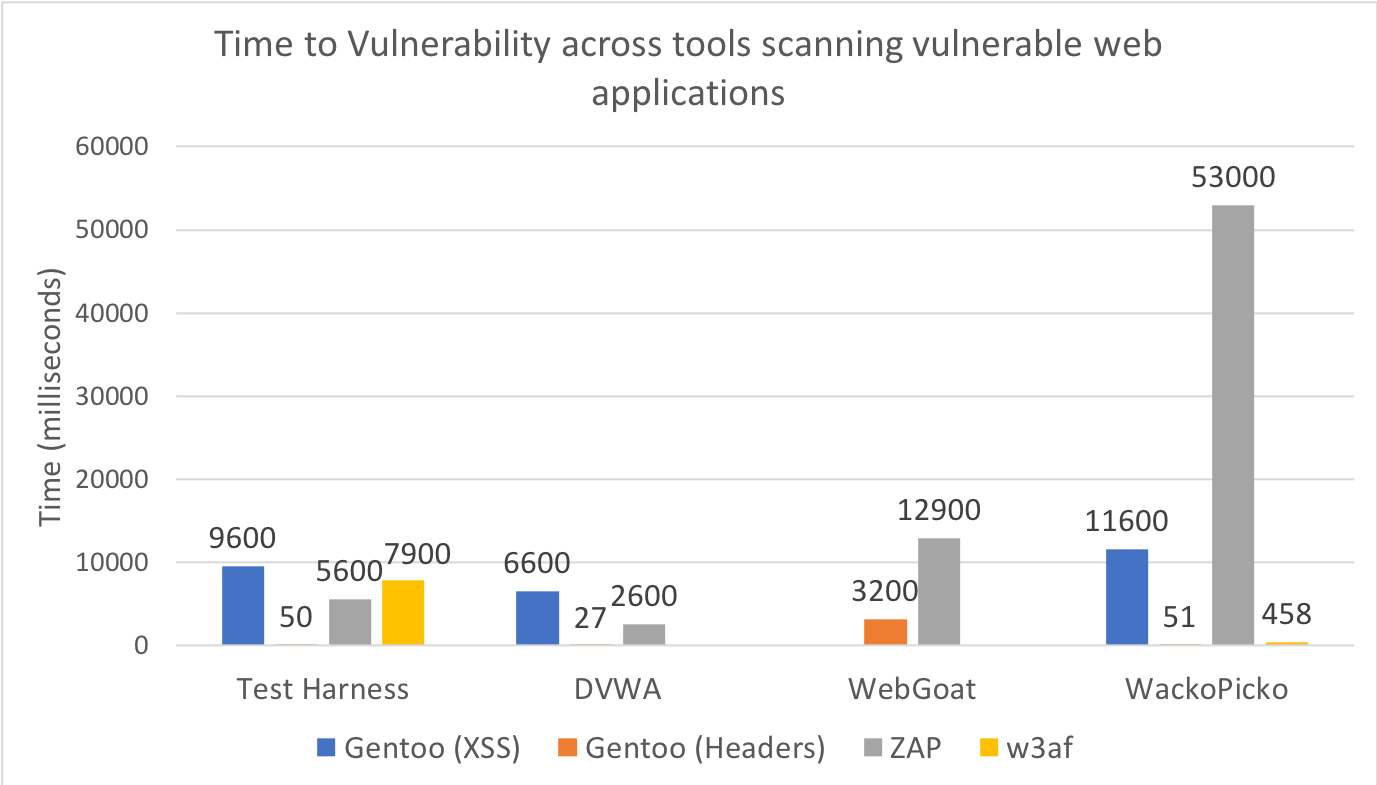
\includegraphics[width=\textwidth]{images/evaluation/time_to_vuln.png}
	\caption{This figure shows the trends across each tool's \textit{Time to Vulnerability} metric}
	\label{fig:time_to_vuln}
\end{figure}

We argue that the numbers presented in Figure \ref{fig:time_to_vuln} are nonetheless qualified to be compared as-is. An argument could be made that these numbers are biased towards Gentoo because the extension is only looking for one type of vulnerability on each scan, whereas ZAP and w3af have to scour the entire application for vulnerabilities. However, it is that very broad scope which ZAP and w3af have access to which counter-balances the argument - both of these tools can search for \textbf{any} possible vulnerability in whichever order they please. This means they can report easier to find vulnerabilities more promptly than Gentoo. That is what we observed with w3af - this tool produces alerts and warnings for some more esoteric vulnerabilities than ZAP and Gentoo, which contributes to its accelerated pace in reporting vulnerabilities (especially notable in the WackoPicko scan). ZAP does not seem to perform as homogeneously as the other tools, but it certainly makes up for this in its consistency and range of vulnerability detections, as shown in the alert figures above. \\

It is pleasing to see that Gentoo has a consistent performance in raw speed of finding a vulnerability from the start of the scan, and that the wait for a specific vulnerability identification is in line with expectations of its user interaction (slower than automatic) and the complexity of the web application. This trend is seen both in the XSS and in the Passive Header scans. \\

We now analyse the \textit{Interaction Volume} for each of the tools, and produce a comparison between these. \\

\begin{figure}[h]
	\centering
	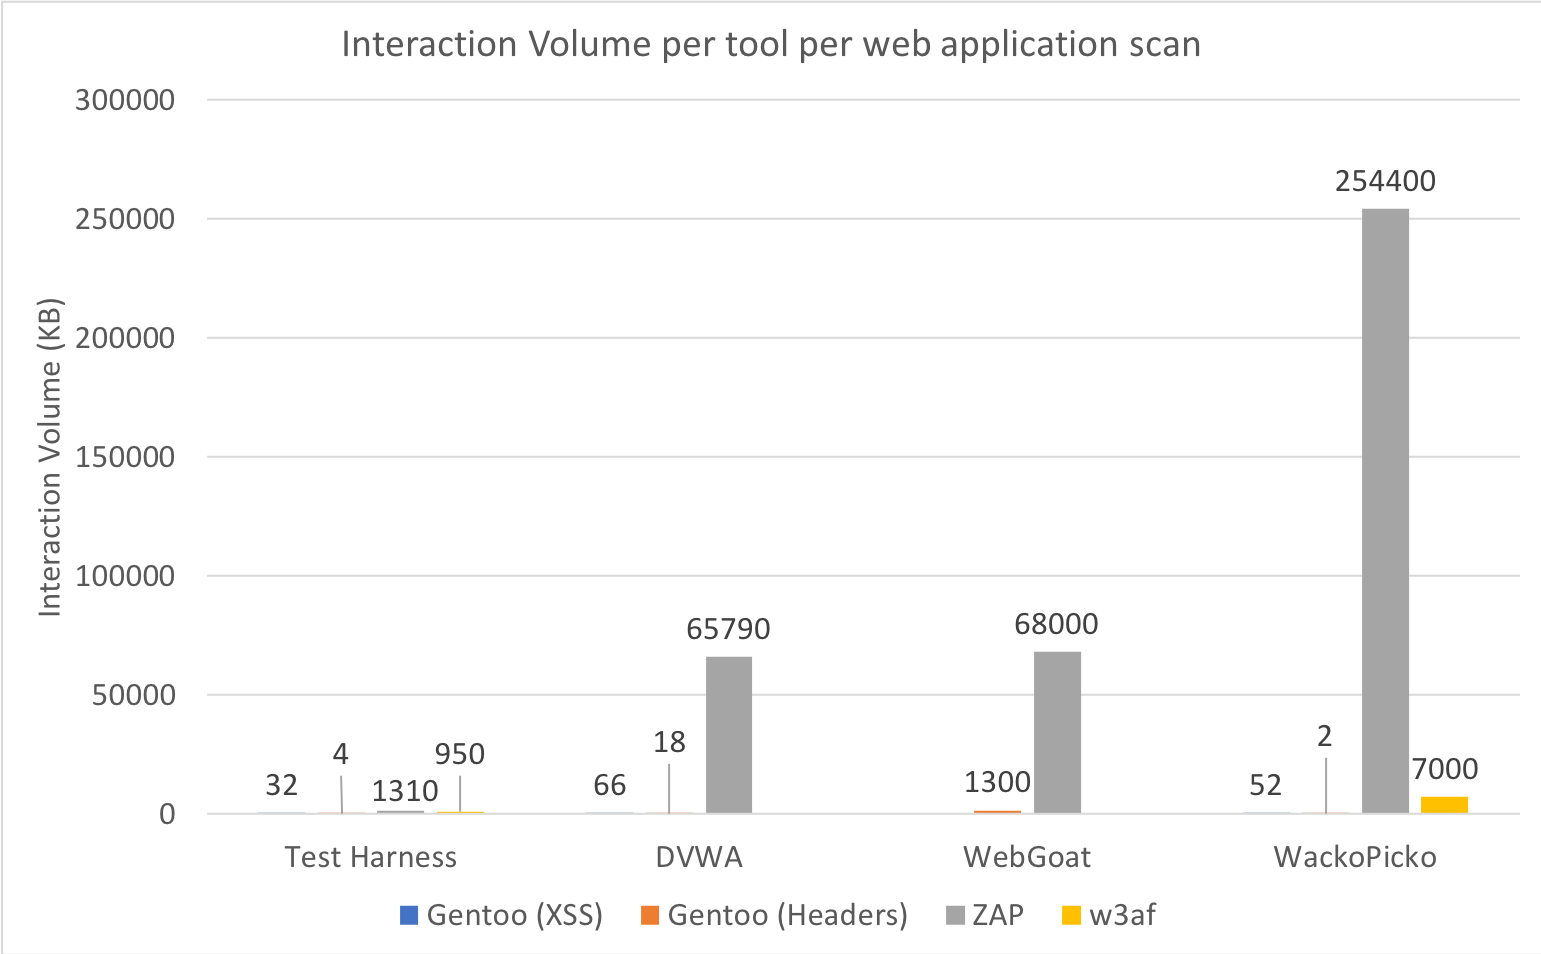
\includegraphics[width=\textwidth]{images/evaluation/interaction_to_volume.png}
	\caption{This figure shows the trends across each tool's \textit{Interaction Volume} metric}
	\label{fig:interaction_volume}
\end{figure}

It is abundantly clear from Figure \ref{fig:interaction_volume} that ZAP has an overwhelmingly larger amount of data transferred in its scans than any of the other tools. In comparison to the others, Gentoo has a consistently small interaction volume in every scan. Unlike the \textit{Time to Vulnerability} metric, the \textit{Interaction Volume} measure is far more dependent on the scanner's scope of attack - the more vulnerabilities a scanner targets, the more requests will have to be sent out (potentially fuzzed) to trigger a wider range of vulnerabilities. As the web application complexity grows, the \textit{Interaction Volume} figures of full-scan tools inflate alongside it, whereas scanning for 1 vulnerability involves attempting the same attack on whatever the surface area presented to attack might be. Therefore, it is reasonable to suggest a normalisation factor for a more apt tool comparison. For the outputs of ZAP and w3af, we divide the \textit{Interaction Volume} by the confirmed number of dangerous vulnerabilities found by each scan to give us the \textit{Normalised Interaction Volume}. This normalised metric should give us a comparison metric that is correlated to the success of the tool - the better it performs in finding vulnerabilities, the lower the \textit{Normalised Interaction Volume}.\\

\begin{figure}[h!]
	\centering
	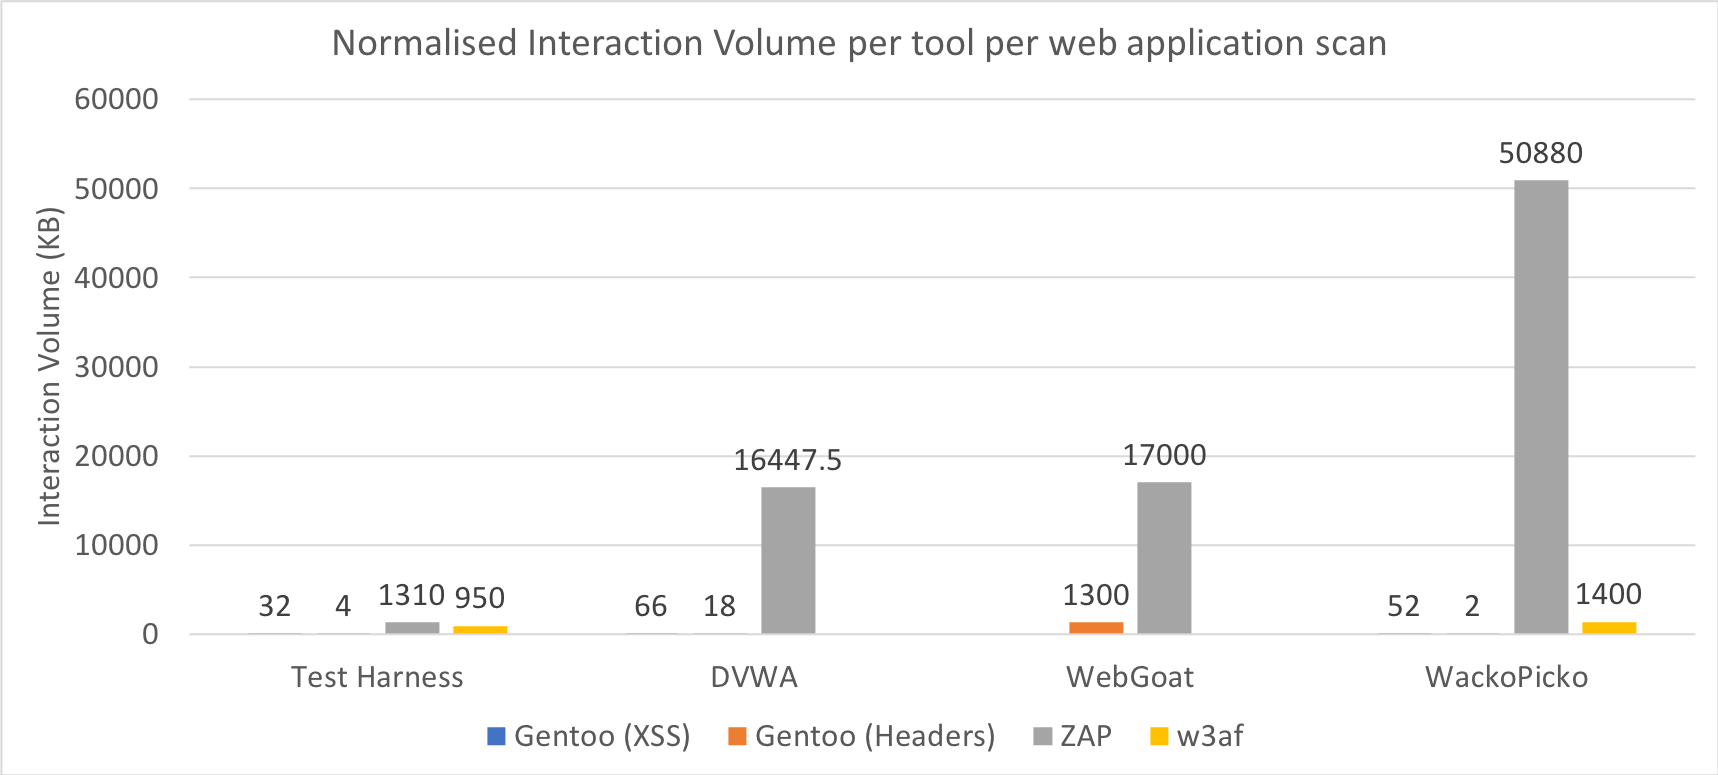
\includegraphics[width=\textwidth]{images/evaluation/normalised_interaction_volume.png}
	\caption{The \textit{Normalised Interaction Volume} mostly affected the figures for ZAP, giving it a fairer means of comparison against Gentoo and w3af}
	\label{fig:normalised_interaction_volume}
\end{figure}

As shown by Figure \ref{fig:normalised_interaction_volume}, the largest change between the \textit{Interaction Volume} and the \textit{Normalised Interaction Volume} metrics is the scale by which ZAP shows a much larger \textit{Interaction Volume} than its competitors (the scale has approximately been divided by 5 from Figure \ref{fig:interaction_volume} to Figure \ref{fig:normalised_interaction_volume}). Clearly, despite the normalisation, ZAP still has an overwhelmingly large amount of \textit{Interaction Volume} when compared to Gentoo and w3af. Gentoo dominates in this category, requiring very little page interactions to successfully fingerprint XSS vulnerabilities. \\

 We see that the \textit{Normalised Interaction Volume} for Gentoo's XSS scan scales with more complex web applications, but in a controlled way, such that it remains the best performer in this category. A low \textit{Normalised Interaction Volume} is desirable as the tool is more likely to remain unnoticed for a longer period of time than its competitors. Web application servers that log requests could easily identify tools such as ZAP and block further requests for fear of Denial of Service or other attack. In a similar situation, Gentoo would remain stealthier for a longer period of time, which is a desirable feature for a penetration tester. \\ 

Lastly, we look at the \textit{Number of replays / attacks needed} (to get to the first vulnerability) for each of the produced scans. As Figure \ref{fig:number_replays_first_vuln} shows, once again, the figures for this metric are heavily skewed when looking at the outputs from ZAP. While Gentoo performs particularly well in this category (with the largest number of replays for any of the scans barely hitting double digits), we can also see that w3af performs reasonably well. \\

\begin{figure}[h!]
	\centering
	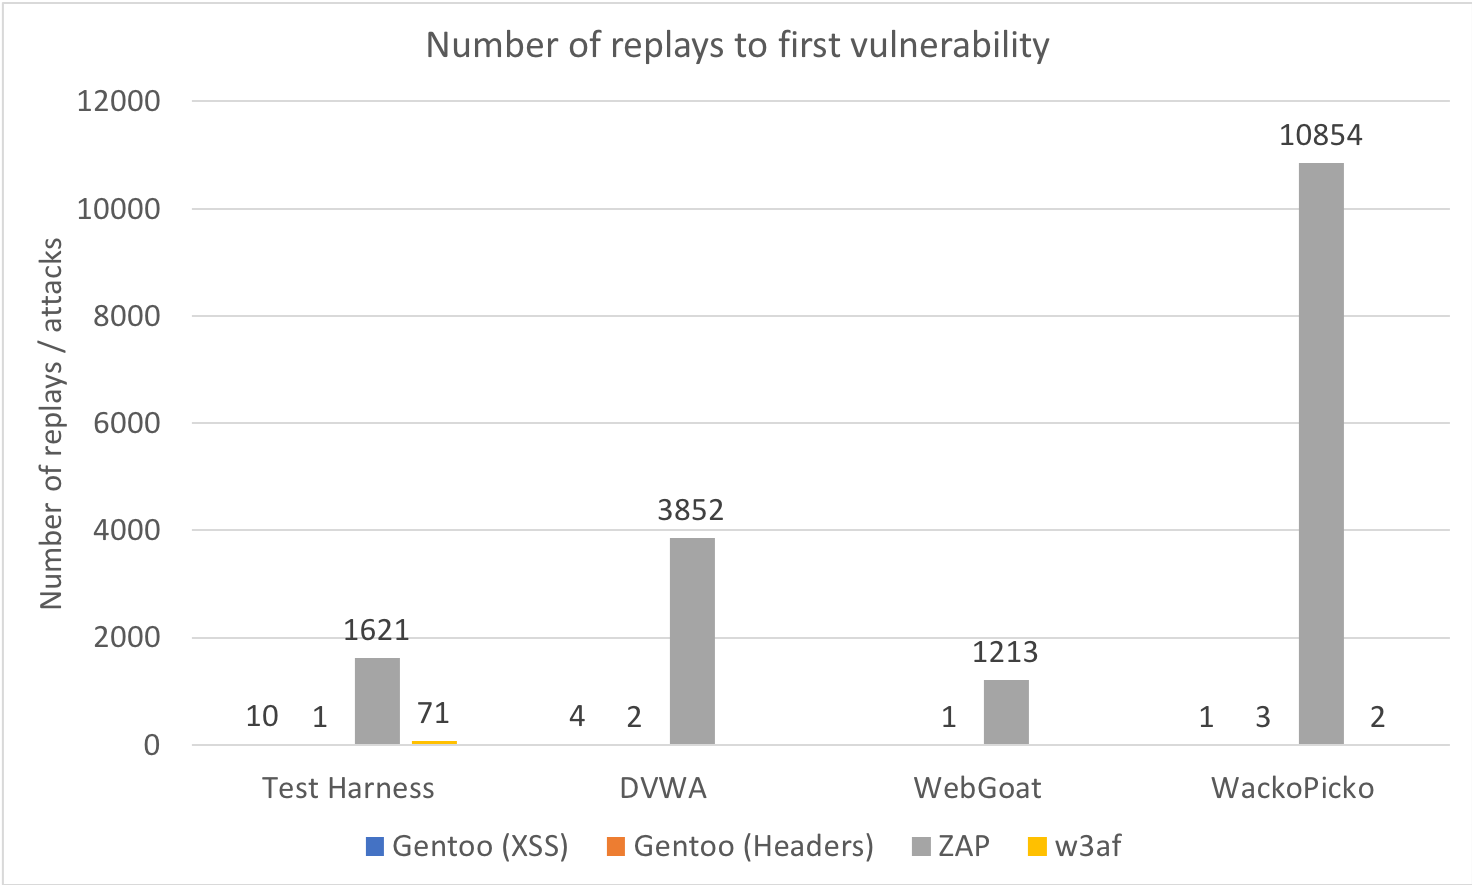
\includegraphics[width=\textwidth]{images/evaluation/number_replays_first_vuln.png}
	\caption{The number of attacks or replays required in a scan to reach the first diagnosed vulnerability}
	\label{fig:number_replays_first_vuln}
\end{figure}


 Clearly, with more requests this metric is easily dilated or distorted - as we have seen from the previous data points, ZAP sends out a far larger number of requests than Gentoo or w3af. Thus we prepare this statistic in a separate way, the percentage of the scan at which the first vulnerability was found (or \textit{Scan completion to first vulnerability}). Instead of measuring how many raw requests are made until a vulnerability is found, it normalizes the data to a percentage of the scan. We see the results in Figure \ref{fig:scan_completion_first_vuln}. \\
 
 \begin{figure}[h!]
 	\centering
 	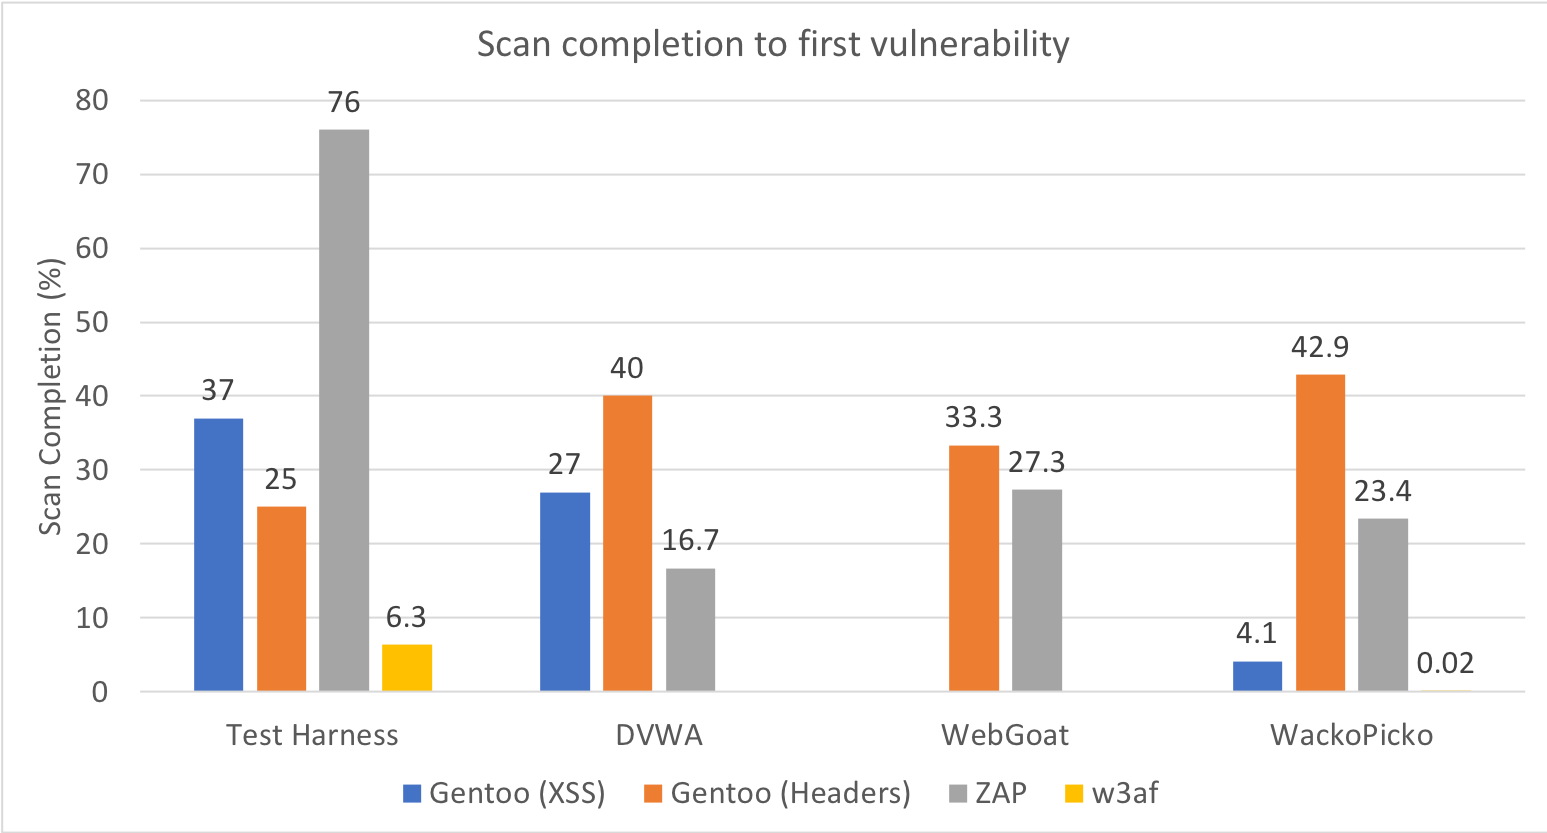
\includegraphics[width=\textwidth]{images/evaluation/scan_completion_first_vuln.png}
 	\caption{The percentage to which the scan was complete when the first vulnerability was found}
 	\label{fig:scan_completion_first_vuln}
 \end{figure}
 
 This metric gives a more interesting basis for analysis. Here, we see that the Gentoo Passive Header scan shows a very stable \textit{scan completion} metric when compared to the other scans. The Gentoo XSS scanner displays positive results here, with all of the \textit{scan completion} results being below 40\%. This leads us to believe that throughout its scans, it detects vulnerabilities with focused attack vectors, making judicious use of its requests. With an even better success rate for this metric, w3af has an extremely low \textit{scan completion} rate, with the worst of the 2 values being under 10\%. This indicates that of the 3 tools, w3af is the best at quickly identifying vulnerabilities, irrespective of their severity. This greedy approach is desirable for pentesters, as this hastily provides them with more information during their \textit{information gathering} phase of testing a web application. \\
 
 Although the \textit{scan completion to first vulnerability} metric provides a more normalized comparison point than the \textit{number of replays / attacks needed to first vulnerability}, it is important to note that it is mathematically skewed to profess superior statistics to scans in which a larger number of requests is sent. In scans with fewer overall requests (namely the Gentoo XSS and Gentoo Headers), each request which is unsuccessful in uncovering a vulnerability counts more towards the \textit{scan completion to first vulnerability} measurement than a similar request for scans which employ more requests overall. In one of the data points (Gentoo Header scan in WebGoat), a total of 3 passive requests were made, of which the first instantly generated an alert which was logged in Gentoo. Despite this seemingly 'perfect' performance for this intended measurement, the \textit{scan completion} metric (correctly) records this at 33\%, which misleads a reader of Figure \ref{fig:scan_completion_first_vuln} into thinking that Gentoo is performing relatively badly. \\
 
 Overall, given the very low numbers reported for the \textit{number of replays / attacks to first vulnerability} as well as the stable numbers for the \textit{scan completion to first vulnerability}, it is fair to deduce that Gentoo has also performed well in this category. This attests that the attacks generated by the extension are executed in a relevant order; attacks that are more likely to uncover vulnerabilities are expected to be ran before other esoteric attacks. \\
 
 In review of the analysis of these metrics between the different tools, we observe the following: 
 
 \begin{itemize}
 	\item ZAP is the most successful of the tools in reporting significant vulnerabilities. This comes at the cost of larger and longer-running scans, which subsequently results in a more conspicuous web application scanner. A large number of requests can more readily identify potential attackers and intruders into an application, which is not desirable for penetration testers (in black-box testing situations).
 	
 	\item w3af produces alerts and warnings for more esoteric vulnerabilities than either ZAP or Gentoo. This tool is also quick to point these out, making it a good option between those analysed for a web analyst in terms of value for time spent.
 	
 	\item Gentoo performed well in all 3 metrics analysed - given that it is only semi-automated, it is still reasonably fast at detecting \textbf{targeted} vulnerabilities. It does so with a small online footprint; we recorded it to have the lowest \textit{normalised interaction volume} of all the tools in the tests. Its attacks are also concise, they quickly detected the intended vulnerabilities as far as the scope of the tests above has shown. The successful performance in these 3 metrics validates the implementation as described in Chapter \ref{implementation}.
 	
 	\item Comparing Gentoo as a human interaction based scanner to fully automated black box scanners is difficult. Different metrics must be analysed in tandem, and we cannot be quick to make absolute judgements on the success or failure of these in comparison to another. 
 \end{itemize}

\section{Live application scanning}

As demonstrated in Section \ref{live_vulnerability}, Gentoo was used as a driving tool behind the uncovering of a real vulnerability on a live website with a significant amount of traffic. The process behind this discovery was very informal - Gentoo's Recommendations feature was often left on after development sessions as we browsed through the internet. We sporadically and (mostly) randomly clicked the recommendations button to see whether Gentoo would be able to uncover any interesting behaviour in websites (at the very least). \\

Indeed, this turned out to be the case. In many websites, triggering Gentoo's Recommendations prompted webpages to produce interesting error pages (some of which revealed relevant information, such as the \texttt{Server} and the \texttt{Powered-By} headers common to many web servers nowadays, as well as versioning information) - in a scenario where a pentester would target these websites, this would be very relevant in the \textit{information gathering} phase. \\

The HTML injection vulnerability detected arose as a result of unexpected behaviour triggered by the recommendations. It was not expected that Gentoo would be used in successfully finding a live vulnerability - this was considered to be an added bonus. The successful identification of this vulnerability thus proved that the implementation of the low effort Recommendations feature was a great success. \\


\section{Accessibility}

Finally, we evaluate different accessibility aspects of the extension. We begin by looking at some compatibility aspects. As we have seen, Gentoo was unable to scan WebGoat due to a scripting error, for reasons we were unable to diagnose. Being incompatible with one of the vulnerable web applications hinders our ability to produce an effective comparison between Gentoo and its competitors. It also highlights what we will call 'creator's bias' - since we have built and tested Gentoo using the Test Harness, the tool becomes overfitted to detecting vulnerabilities in this web application. Thus, when we eventually test the extension against other applications, due to lack of testing or programming generalisation, as seen with WebGoat, the extension is unable to scan for vulnerabilities. This also explains the reason as to why Gentoo was unable to detect the Persisted XSS vulnerability within DVWA. Although the \texttt{textarea} HTML tag is a valid form input, it was not included in the Test Harness. As a result, Gentoo's Action Replay algorithm does not check for additional inputs submitted through \texttt{textarea} - meaning it skips out on detecting an important vulnerability. \\

One of ZAP's most useful features is being able to open a browser window at the URL which is being attacked. While it is open, ZAP logs the user's input, including any credentials used in form submissions, to help with crawling the web application. This feature is not present in w3af, making it very reliant on its own authentication mechanisms. These were difficult and unreliable to setup, meaning w3af was effectively unable to scan both DVWA and WebGoat. In comparison, Gentoo has no need for this feature because it is inherent to how the browser extension functions - the program has direct access to the web application, and effectively acts as a middle-man between it and the user. The user does not need to worry about crawling nor authentication beyond their own account, because Gentoo acts as a companion, analysing whatever website the user decides to browse. Thus Gentoo incorporates one of the most useful features in web app scanners by default, massively improving its usability. \\

As part of development, we have created a user feedback form for interested people who were willing to partake in a small experiment to gather data on how users used Gentoo. Although this experiment has not yet gathered enough data for statistical relevance, some of the user feedback regarding usability is useful to consider. While observing users attempt to uncover the XSS vulnerability using Gentoo on the Test Harness, it became clear that of all the mechanisms in the extension, using the Action Replay mode was particularly unclear. Although there are some limited instructions written in plaintext in the popup page regarding usage, users were still confused about how to use the Action Replay, and made no progress in uncovering vulnerabilities on their own when using this mode. Thus, accessibility for users in Gentoo could have been improved by adding a guided tutorial or a plaintext page with instructions on how to use the extension itself. \\ 






